\documentclass[conference]{IEEEtran}
\usepackage{cite}
\usepackage{amsmath,amssymb,amsfonts}
\usepackage{graphicx}
\usepackage{float}
\usepackage{url}
\usepackage[hidelinks]{hyperref}
\usepackage{textcomp}
\usepackage{enumitem}
\usepackage{booktabs}
\usepackage{siunitx}
\usepackage[caption=false,font=footnotesize]{subfig}
\graphicspath{{source/extracted_images/}}

\begin{document}

\title{Integrated Symbolic Planning and Robotic Execution: A PDDL-Based Task Planner with ROS~2 and Gazebo}

\author{
\IEEEauthorblockN{Andrew Khalil Abdelmalak}
\IEEEauthorblockA{\textit{Dept. of Mechatronics Engineering} \\
\textit{German University in Cairo (GUC)}\\
Cairo, Egypt}
\and
\IEEEauthorblockN{Daniel George Boules}
\IEEEauthorblockA{\textit{Dept. of Mechatronics Engineering} \\
\textit{German University in Cairo (GUC)}\\
Cairo, Egypt}
\and
\IEEEauthorblockN{David Louis Girgis}
\IEEEauthorblockA{\textit{Dept. of Mechatronics Engineering} \\
\textit{German University in Cairo (GUC)}\\
Cairo, Egypt}
\and
\IEEEauthorblockN{Samir Sameh Yacoub}
\IEEEauthorblockA{\textit{Dept. of Mechatronics Engineering} \\
\textit{German University in Cairo (GUC)}\\
Cairo, Egypt}
\and
\IEEEauthorblockN{Youssef Youssry}
\IEEEauthorblockA{\textit{Dept. of Mechatronics Engineering} \\
\textit{German University in Cairo (GUC)}\\
Cairo, Egypt}
}

\maketitle

\begin{abstract}
This paper presents the design and implementation of an integrated symbolic planning and robotic execution system for autonomous mobile manipulation. A PDDL-based task planner using Fast Downward with A* search and the LM-Cut heuristic generates action plans from high-level goals, which are then translated into physical robot commands through a modular ROS~2 architecture. The system operates a TurtleBot3 with an OpenManipulator arm in the Gazebo simulation environment, performing autonomous navigation via Nav2 and object manipulation through sequential gripper control. A Knowledge Base (KB) is updated in closed-loop fashion only after successful physical execution, ensuring state consistency between the symbolic and physical layers. Experimental results demonstrate successful end-to-end task completion, including multi-room navigation with 0.30\,m tolerance and pick-and-place manipulation sequences.
\end{abstract}

\begin{IEEEkeywords}
Task planning, PDDL, ROS~2, mobile manipulation, TurtleBot3, Gazebo, Nav2, symbolic AI, autonomous robotics.
\end{IEEEkeywords}

\section{Introduction}

Autonomous robotic systems that can reason about high-level goals and translate them into low-level physical actions represent a central challenge in AI for robotics~\cite{ghallab2004}. While classical robotics excels at motion planning and control, bridging the gap between symbolic reasoning and continuous robot execution remains an active research area~\cite{kaelbling2011}.

This work addresses the integration challenge by combining three key capabilities:
\begin{itemize}
\item \textbf{Symbolic Planning:} A PDDL-based planner (Fast Downward~\cite{helmert2006}) generates action sequences from declarative goal specifications.
\item \textbf{Plan Translation:} A bridge layer maps symbolic actions (e.g., \texttt{move~kitchen}) to continuous ROS~2 commands with appropriate coordinates and tolerances.
\item \textbf{Physical Execution:} The TurtleBot3 with OpenManipulator autonomously navigates between rooms using Nav2 and manipulates objects using sequential gripper control.
\end{itemize}

A critical design decision is the closed-loop Knowledge Base (KB) update: the symbolic state is modified only after confirmed physical execution, preventing plan-reality divergence~\cite{ingrand2017}.

\section{System Architecture}

\subsection{World Model}

The environment models a multi-room apartment with six rooms, each assigned navigation coordinates within the Gazebo House World (Table~\ref{tab:rooms}).

\begin{table}[H]
\centering
\caption{Room Coordinates in Gazebo World Frame}
\label{tab:rooms}
\begin{tabular}{lcc}
\toprule
\textbf{Room} & \textbf{x (m)} & \textbf{y (m)} \\
\midrule
Storage & $-4.5$ & $-1.5$ \\
Living Room & $-1.0$ & $1.5$ \\
Dining Room & $6.0$ & $1.0$ \\
Bathroom & $3.0$ & $5.0$ \\
Bedroom & $-4.5$ & $3.5$ \\
Kitchen & $8.5$ & $-1.5$ \\
\bottomrule
\end{tabular}
\end{table}

Ten objects are distributed across rooms (e.g., cup in kitchen, book in bedroom) and tracked in a Python KB that synchronizes with the PDDL problem definition.

\subsection{PDDL Domain Specification}

The symbolic layer uses the following predicates: \texttt{robot-at(r)}, \texttt{at(o,r)}, \texttt{handempty()}, \texttt{holding(o)}, and \texttt{connected(r1,r2)}. Three action schemas define the planning operators:

\begin{itemize}[nosep, leftmargin=1.5em]
\item \texttt{\textbf{Move(from, to)}}: Preconditions: \texttt{robot-at(from)}, \texttt{connected(from,to)}. Effects: \texttt{robot-at(to)}, $\neg$\texttt{robot-at(from)}.
\item \texttt{\textbf{Pick(o, r)}}: Preconditions: \texttt{robot-at(r)}, \texttt{at(o,r)}, \texttt{handempty}. Effects: \texttt{holding(o)}, $\neg$\texttt{at(o,r)}, $\neg$\texttt{handempty}.
\item \texttt{\textbf{Place(o, r)}}: Preconditions: \texttt{robot-at(r)}, \texttt{holding(o)}. Effects: \texttt{at(o,r)}, $\neg$\texttt{holding(o)}, \texttt{handempty}.
\end{itemize}

\subsection{Planning Engine}

The planner uses Fast Downward~\cite{helmert2006} with A* search and the LM-Cut heuristic, producing optimal action sequences. Fig.~\ref{fig:cli_init} shows the CLI interface with the initial KB state, while Fig.~\ref{fig:plan_exec} demonstrates a complete plan for the goal \texttt{at~cup~storage}.

\begin{figure}[H]
\centering
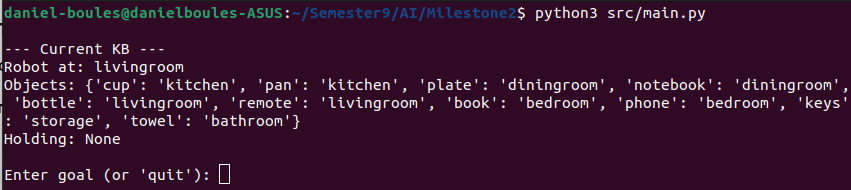
\includegraphics[width=\columnwidth]{page4_img1.jpeg}
\caption{CLI interface showing the initial Knowledge Base state: robot in the living room, ten objects distributed across six rooms.}
\label{fig:cli_init}
\end{figure}

\begin{figure}[H]
\centering
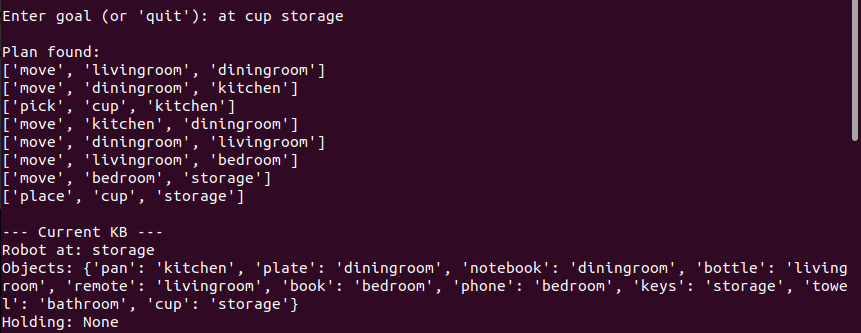
\includegraphics[width=\columnwidth]{page4_img2.jpeg}
\caption{Plan execution for goal ``at cup storage'': the planner generates an 8-step sequence (six \texttt{move}, one \texttt{pick}, and one \texttt{place}) traversing five rooms. The KB updates after each confirmed action.}
\label{fig:plan_exec}
\end{figure}

\section{ROS~2 Integration}

\subsection{Architecture Overview}

The execution pipeline consists of three layers:
\begin{enumerate}
\item \textbf{Plan Executor} (\texttt{executor.py}): Parses PDDL actions and launches appropriate ROS~2 nodes via Python subprocesses.
\item \textbf{Navigation Node}: Interfaces with the Nav2 stack, sending target coordinates as \texttt{/navigate\_to\_pose} action goals with a configurable tolerance of 0.30\,m.
\item \textbf{Gripper Node}: Controls the OpenManipulator via \texttt{/arm\_controller/\allowbreak follow\_joint\_trajectory} and \texttt{/gripper\_controller/\allowbreak gripper\_cmd}, implementing a three-phase manipulation sequence.
\end{enumerate}

Table~\ref{tab:ros_interfaces} summarizes the key ROS~2 interfaces.


\begin{table}[H]
\centering
\caption{Key ROS~2 Interfaces}
\label{tab:ros_interfaces}
\begin{tabular}{llc}
\toprule
\textbf{Component} & \textbf{Type} & \textbf{Topic/Action} \\
\midrule
Navigation & Action Client & \texttt{/navigate\_to\_pose} \\
Arm Control & Action Client & \texttt{/arm\_controller/...} \\
Gripper & Action Client & \texttt{/gripper\_controller/...} \\
\bottomrule
\end{tabular}
\end{table}

\subsection{Launch Configuration}

Two launch files orchestrate the simulation:
\begin{itemize}
\item \textbf{Gazebo Launch}: Loads the TurtleBot3 house environment, spawns the robot model at configurable coordinates, and publishes TF transforms. The repository also provides a custom apartment world (\texttt{my\_house.world}, model \texttt{tb3\_house\_custom}) in \texttt{ros/tb3\_course\_assets/}.
\item \textbf{Navigation Launch}: Brings up the Nav2 stack~\cite{nav2} (AMCL localizer, global/local planners), loads the custom SLAM occupancy grid (\texttt{map.yaml}), and starts RViz2 for visualization.
\end{itemize}

\section{Experimental Results}

\subsection{Navigation Performance}

The robot successfully navigated between all room pairs using Nav2's global planner (Fig.~\ref{fig:navigation}). The 0.30\,m positional tolerance prevents oscillatory behavior near goal positions while maintaining sufficient accuracy for the symbolic room-level abstraction.

\begin{figure}[H]
\centering
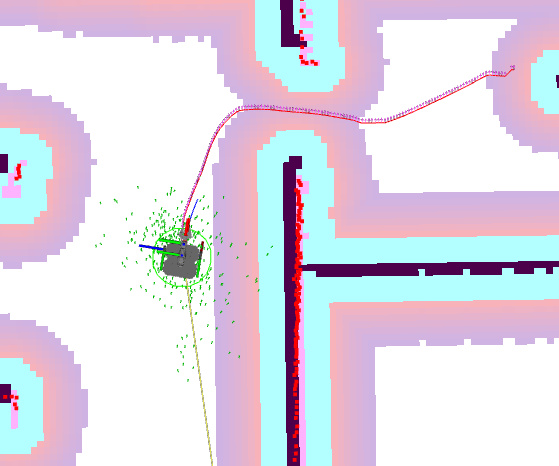
\includegraphics[width=\columnwidth]{page8_img1.jpeg}
\caption{Navigation execution in RViz: the global planner (red line) generates a path from the Dining Room to the Kitchen, overlaid on the costmap. The robot (center) with LIDAR scan (green) successfully follows the planned trajectory.}
\label{fig:navigation}
\end{figure}

\subsection{Manipulation Sequence}

Object manipulation follows a three-phase sequence validated in Gazebo (Fig.~\ref{fig:manipulation}):
\begin{enumerate}
\item \textbf{Approach:} Arm lowers to pre-set pick/place coordinates.
\item \textbf{Actuate:} Gripper opens (place) or closes (pick) based on the PDDL action.
\item \textbf{Retract:} Arm returns to the safe driving home pose.
\end{enumerate}

\begin{figure}[H]
\centering
\subfloat[Arm down]{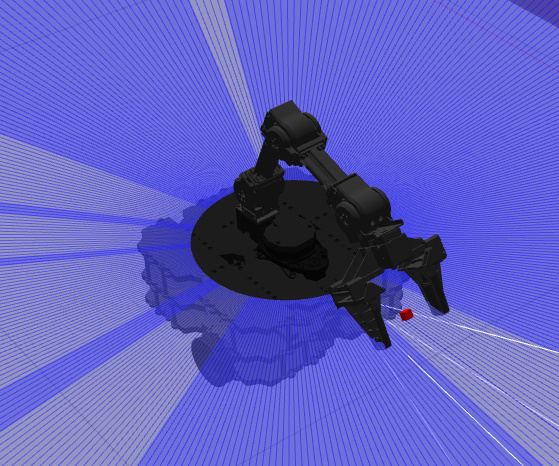
\includegraphics[width=0.31\columnwidth]{page8_img2.jpeg}}
\hfill
\subfloat[Actuate]{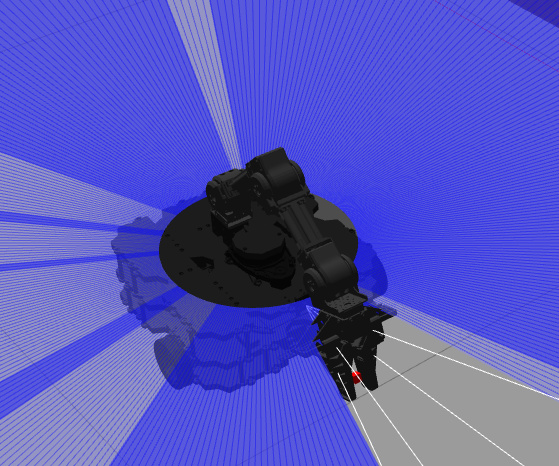
\includegraphics[width=0.31\columnwidth]{page8_img3.jpeg}}
\hfill
\subfloat[Home pose]{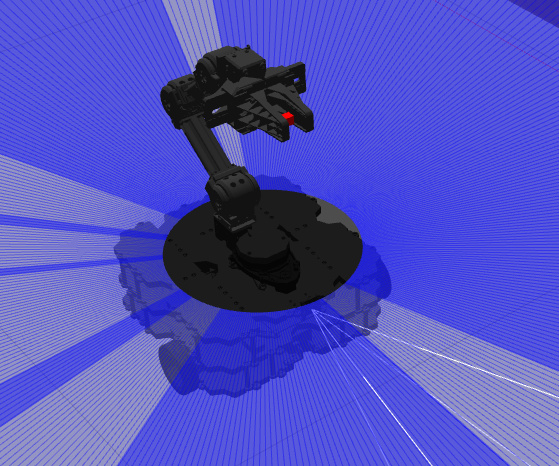
\includegraphics[width=0.31\columnwidth]{page8_img4.jpeg}}
\caption{Three-phase manipulation sequence in Gazebo: (a)~arm lowers to approach position, (b)~gripper actuates (open/close), (c)~arm returns to safe home pose for driving.}
\label{fig:manipulation}
\end{figure}

\subsection{End-to-End Task Completion}

We tested the integrated system with the goal \texttt{at~cup~storage}, requiring:
\begin{itemize}
\item Navigation across 5 rooms via 6 move actions (livingroom $\to$ diningroom $\to$ kitchen $\to$ diningroom $\to$ livingroom $\to$ bedroom $\to$ storage).
\item One pick action in the kitchen and one place action in storage.
\item KB updated only after each physical action succeeds.
\end{itemize}

\section{Discussion}

The closed-loop KB update strategy proved essential for system reliability. By deferring symbolic state changes until physical execution confirms success, the system avoids the ``plan divergence'' problem common in open-loop execution architectures~\cite{ingrand2017}.

The 0.30\,m navigation tolerance represents a pragmatic trade-off: tighter tolerances caused oscillation near goals, while looser tolerances risked the robot stopping outside rooms. The room-level symbolic abstraction means exact positioning is less critical than reliable arrival.

Limitations include the absence of visual object detection (objects are assumed at known positions) and the lack of re-planning capability on execution failure. Integrating computer vision for object localization and failure recovery would significantly enhance system robustness.

\section{Conclusion}

We demonstrated a complete pipeline from symbolic AI planning to physical robotic execution. By connecting a Fast Downward PDDL planner to the ROS~2 ecosystem via a modular execution bridge, the TurtleBot3 with OpenManipulator autonomously navigates a multi-room environment and performs pick-and-place tasks based on high-level goal specifications. The closed-loop KB architecture ensures state consistency between symbolic reasoning and physical reality.

\begin{thebibliography}{5}

\bibitem{ghallab2004}
M.~Ghallab, D.~Nau, and P.~Traverso, \emph{Automated Planning: Theory and Practice}.\hskip 1em plus 0.5em minus 0.4em Morgan Kaufmann, 2004.

\bibitem{kaelbling2011}
L.~P. Kaelbling and T.~Lozano-P\'{e}rez, ``Hierarchical task and motion planning in the now,'' in \emph{Proc. IEEE Int. Conf. Robotics and Automation (ICRA)}, 2011, pp.~1470--1477.

\bibitem{helmert2006}
M.~Helmert, ``The Fast Downward planning system,'' \emph{J. Artificial Intelligence Research}, vol.~26, pp.~191--246, 2006.

\bibitem{ingrand2017}
F.~Ingrand and M.~Ghallab, ``Deliberation for autonomous robots: A survey,'' \emph{Artificial Intelligence}, vol.~247, pp.~10--44, 2017.

\bibitem{nav2}
S.~Macenski, F.~Mart\'{i}n, R.~White, and J.~G. Crespo, ``The Marathon 2: A navigation system,'' in \emph{Proc. IEEE/RSJ Int. Conf. Intelligent Robots and Systems (IROS)}, 2020.

\end{thebibliography}

\end{document}
